\section{Results and analysis}
The algorithm has been tested upon the same data used by the researchers in \cite{fire_distinguish}. More precisely, the used data correspond to the fire occurred in Huzhong, region located in
Mt. Daxing’anling, at $10:40$ local time on June 29, 2010. The flames hit a total of 7 fire points in that specific area. \\
For the purposes of this work, the researchers reported all the necessary parameters to calculate the objective functions. The only element that's missing is the upper bound to the number
of vehicles for each fire point ($U_i$). Since in the paper it was presented as a given parameters, we used a representative number $10$ for all the points.\\
In Table \ref{tab:our_solutions} we reported the results obtained after running the algorithm 4 consecutive times. The lowest calculated time to extinguish all
the fires is $6.17$ hours, using all the vehicles, while the lowest number of vehicles used is $29$, that is the lower bound given by the authors. In the latter case, the extinguish
time is $40.04$ hours. In figure \ref{fig:pareto_results} these solutions are plot on a 2D graph with $f_1$ on the $x$ axis and $f_2$ on the $y$ axis. 
We can see that most of the solutions are concentrated between 5 and 20 hours for $f_1$ and these solutions cover almost all the values in $f_2$, so the results are satisfying. 
Our results are very similar to the ones found by the authors, however the pareto front in their experiment (Fig. \ref{fig:authors_results}) is very well distributed and 
all the runs produce very similar solutions.

\begin{figure}
    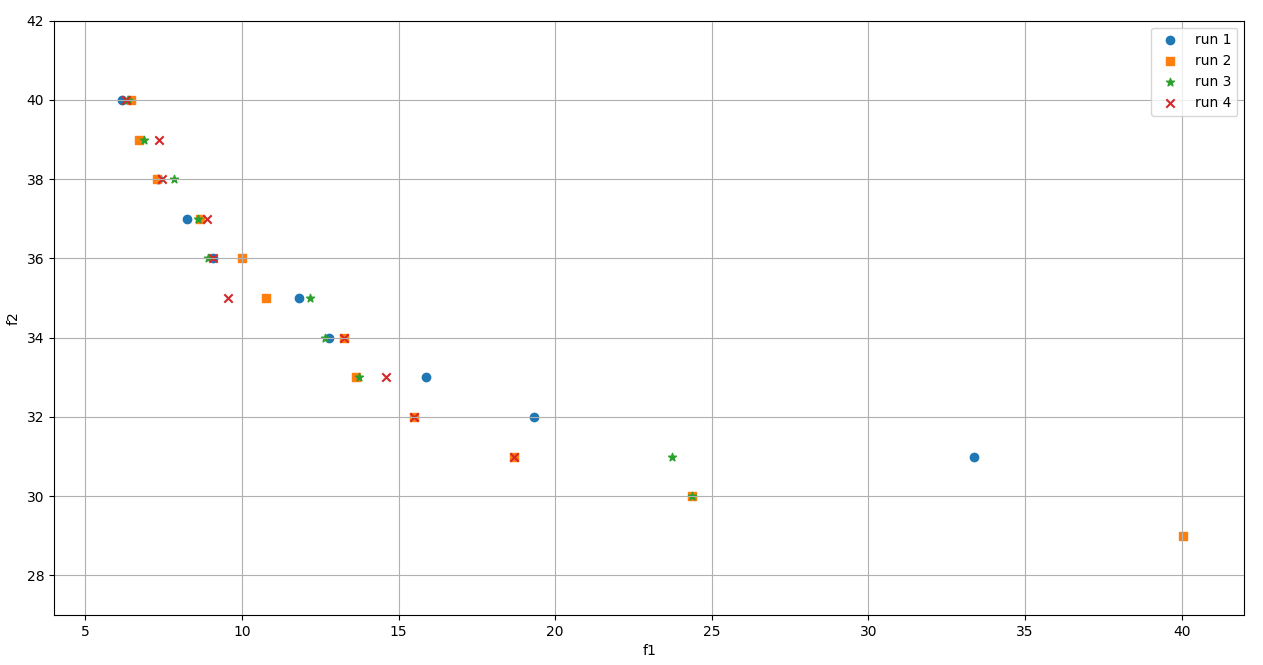
\includegraphics[width=\linewidth]{Images/our_results_4_runs.png}
    \caption{Our Pareto solutions}
    \label{fig:pareto_results}
\end{figure}

\begin{figure}
    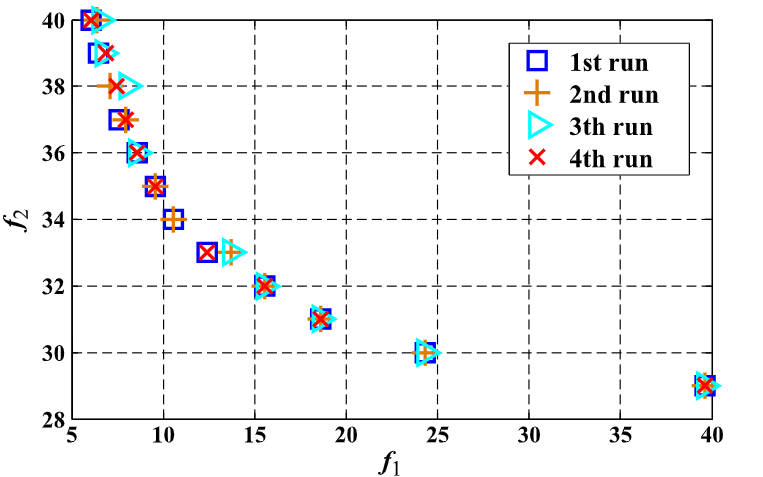
\includegraphics[width=\linewidth]{Images/authors_results.png}
    \caption{Authors' Pareto solutions}
    \label{fig:authors_results}
\end{figure}
